\documentclass[11pt,a4paper]{article}

\usepackage[utf8]{inputenc}
\usepackage[english]{babel}
\usepackage[T1]{fontenc}
\usepackage{graphicx}
\usepackage{bm}
\usepackage[colorlinks=true]{hyperref}
\usepackage{mathtools}
\usepackage{slashbox}

\usepackage{amsmath,amssymb,amsfonts,amsthm}
\newcommand{\mbf}[1]{\bm{#1}}
\newcommand{\mono}[1]{\texttt{#1}}
\DeclareMathOperator{\sgn}{sgn}

\newcommand*{\matminus}{%
  \leavevmode
  \hphantom{0}%
  \llap{%
    \settowidth{\dimen0 }{$0$}%
    \resizebox{\dimen0 }{\height}{$-$}%
  }%
}

% Only number equations that have references to them
\mathtoolsset{showonlyrefs}

\title{Assignment 3}
\author{Sebastian Paaske Tørholm \& Kristoffer Søholm \& Søren Dahlgaard}

\begin{document}
\maketitle

\section{Question 1.1}

We wish to show that the derivative of the activation function is given by
\[
    \frac{d}{da} \frac{a}{1+|a|} = \frac{1}{(1+|a|)^2}\ .
\]
For $a\ge 0$ we have
\[
    f(a) = g(a)h(a)\ ,
\]
with $g(a) = a$ and $h(a) = (1+a)^{-1}$. We also have $g'(a) = 1$ and
$h'(a) = -(1+a)^{-2}$. By the product rule we get
\begin{align}
    f'(a) &= g'(a)h(a) + g(a)h'(a) \\
          &= \frac{1}{1+x} - \frac{x}{(1+x)^2} \\
          &= \frac{1+x}{(1+x)^2} - \frac{x}{(1+x)^2}\ .
\end{align}
For $a < 0$ we instead have $h(a) = (1-a)^{-1}$. Using the same approach and
combining the results, we arrive at
\[
    f'(a) =
    \begin{cases}
        1/(1+x)^2 & \text{if $x\ge 0$} \\
        1/(1-x)^2 & \text{if $x < 0$}
    \end{cases}
\]
as desired.

In our implementation of the feed forward network and the backpropagation
algorithm, we have followed the method described in \cite{ufldl}. This was
more intuitive to us.

We wish to use the mean-squared error (MSE) as our error function. This is
given by
\[
    E(w) = \frac{1}{m} \sum_{i=1}^m (y(w, x_i) - t_i)^2\ .
\]
This error function is implemented in the file \mono{ffneterror.m}. We note,
that backpropagation minimizes the sum-of-squares error function, which is
not the same as the MSE. However, the two error functions only differ by a
constant factor of $2/m$, so we can multiply the backpropagation result by
this to obtain the gradient that corresponds to the MSE function. Our
implementation of the feed-forward neural network can be seen in
\mono{ffnet.m}, and the implementation of backwards propagation can be seen
in \mono{backprop.m}. In \mono{assignment3.m} we compare the initial gradient
computed with the numerical approach (\mono{numgrads.m}) and using backwards
propagation. With $\varepsilon = 1e-6$ the difference between the two
approaches was around $10^{-6}$, which is reasonable. Note, that we initialize
the values of $w$ randomly according to a gaussian, so the error is not the
same on every run.


\section{Question 1.2}
Training of the neural network is implemented in the function \mono{train.m}.
It runs for a set number of iterations rather than using some stop criterium.
The reason is that training the network is quite computational intensive, so
we would like to be certain that it stops at some point.

The trainer uses a simple steepest descent, and does not use any form of
early-stopping or weight decay to avoid over fitting. It is clear that both of
these could be used to avoid over-fitting. As mention in \cite{Bishop}, the
error function w.r.t the training set decreases with the number of iteration,
but at some point, the network will start to overfit. By measuring the error
w.r.t a validation set as well, we are able to stop before overfitting becomes
a problem.

We used a learning rate of $\alpha = 0.3$ to produce the results below. In
general we found that using too small learning rates made the training very
slow, as many more iterations were needed. Using too big learning rates
caused the optimizer to ``jump too far'', which caused some weird spikes in
MSE for the different iterations. It could actually lead to a worsening in the
error function. This issue could be solved by performing a line search along
the direction of the negative gradient instead of using a fixed learning rate.

\autoref{fig:func} shows the original data samples, the sinc function and
the evaluated neural networks for the interval $[-10, 10]$. The blue line
corresponds to the network with $2$ hidden neurons, and the green line is the
network with $20$ hidden neurons. It is clear that both networks have problems
with capturing the sinc function on the left, and perform slightly better
on the right. It is quite clear, that the network with more neurons was better
at approximating the function.

\begin{figure}[htbp]
    \centering
    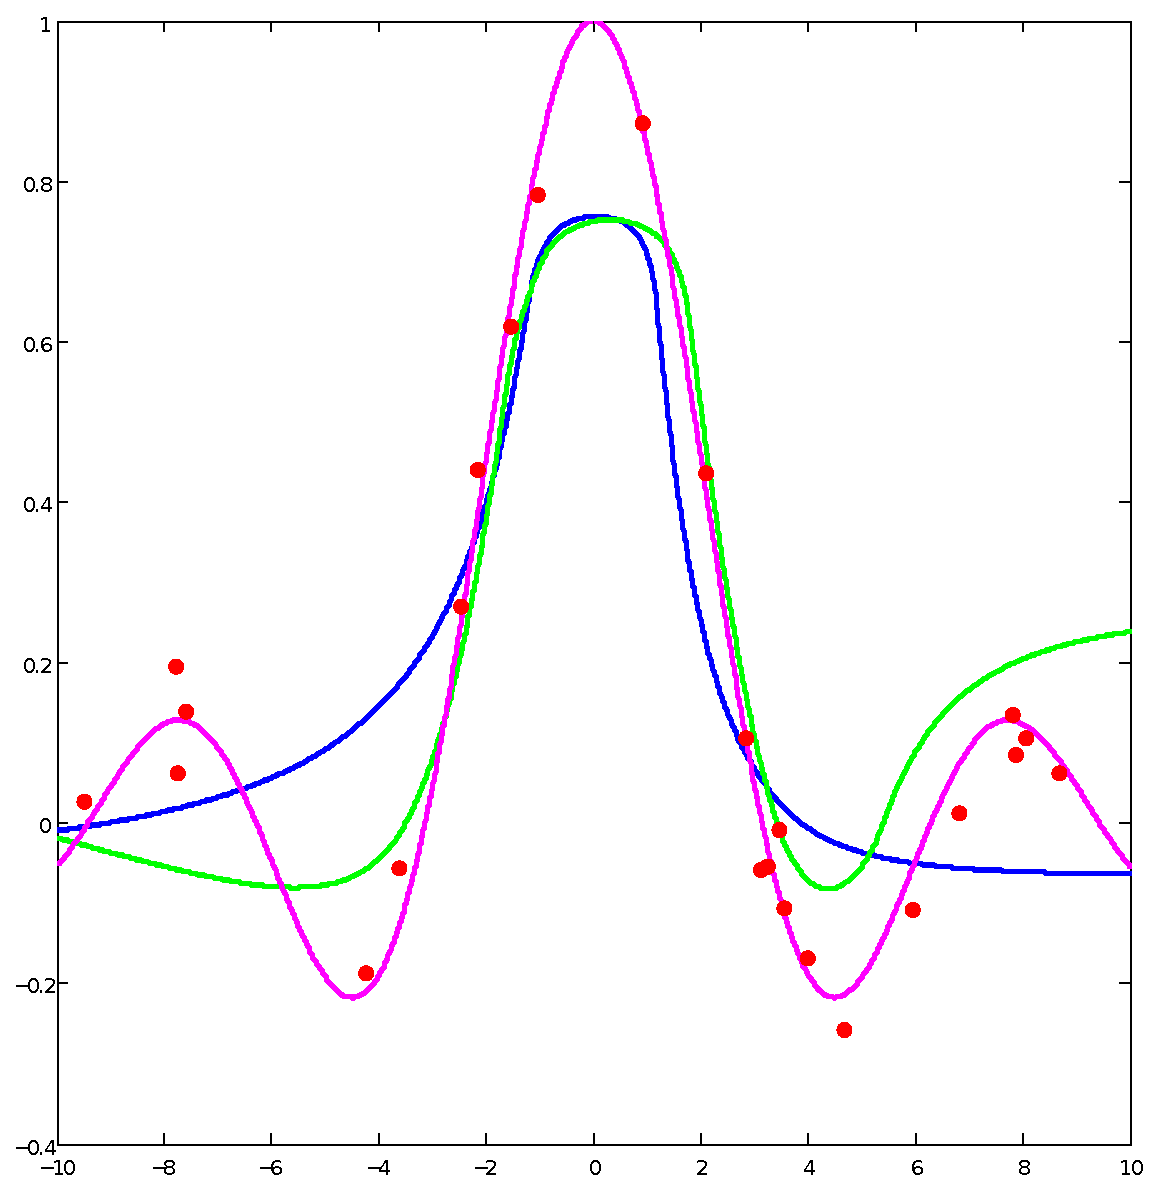
\includegraphics[width=\textwidth]{figures/functions.pdf}
    \caption{The training samples, sinc function and the two neural networks
        plotting along with each other. The blue and green curves correspond
    to the networks with $2$ and $20$ hidden neurons respectively.}
    \label{fig:func}
\end{figure}

\autoref{fig:error_norm} shows the MSE of the networks and the
norm of the gradients (another common stopping criteria) per iteration. This
figure suggests, that the learning rate we used was probably a bit too big,
which is evident from the spiky curve of the MSE. It is very interesting to
note the behaviour of the gradient, which seems very counter intuitive. We
would expect the gradient to become smaller and smaller during the
optimization like it does for the small network. This is definitely not the
case for the big network, which is very odd. We
have no idea as to what may be causing this. A possible fix to this behaviour
could be to add a weight-decay term to the error function which gradient we
compute. The size of the gradient for the big network is also a reason why we
cannot use as big a learning rate for it as we wish to.

\begin{figure}[htbp]
    \centering
    \begin{minipage}[b]{\linewidth}
        \centering
        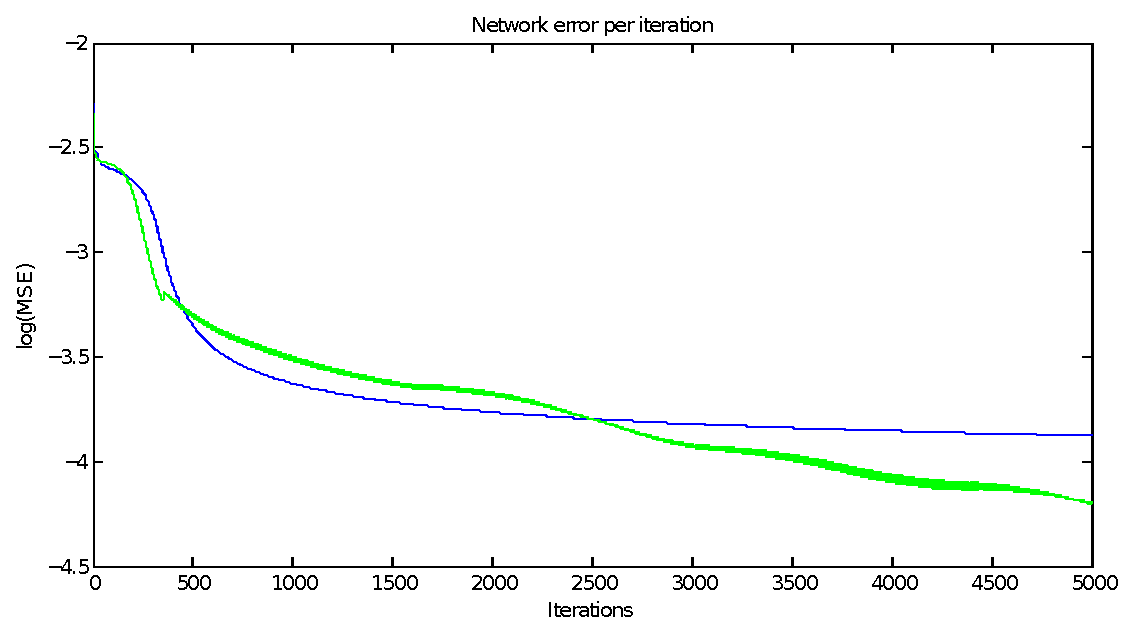
\includegraphics[width=\textwidth]{figures/errors.pdf}
    \end{minipage}

    \begin{minipage}[b]{\linewidth}
        \centering
        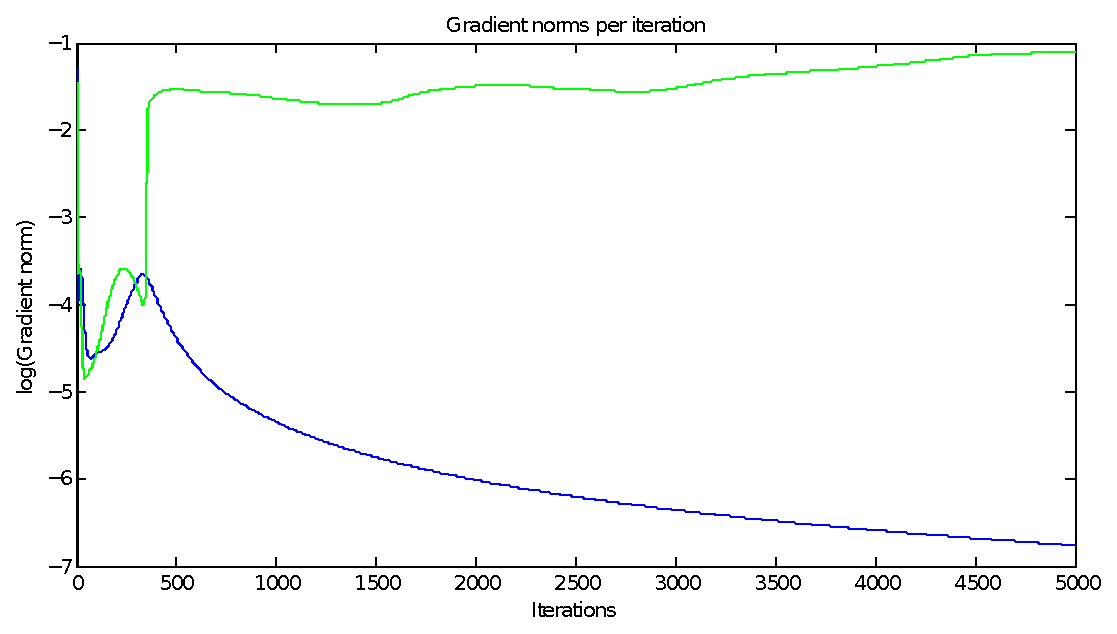
\includegraphics[width=\textwidth]{figures/norms.pdf}
    \end{minipage}
    \caption{The MSE and the norm of the gradient for the two neural networks
        during the training. The blue line corresponds to the network with $2$
    hidden neurons, and the green line to the one with $20$ hidden neurons.}
    \label{fig:error_norm}
\end{figure}

\section{Question 2.1}
To normalize the data we use the affine linear mapping, which transforms each index $x_i$ to

$$ f_{norm}(x_i) = \frac{x_i - \mu}{\sigma^2} $$

Before the normalization we have the following values for the mean and variance of the training data:
\begin{align}
\mu_{train} =  (&155.9603,204.8211,115.0586,0.0059,4.2887e\matminus05,0.0032,0.0033, \\
                &0.0096,0.0277,0.2624,0.0146,0.0166,0.0219,0.0440,0.0226, \\
                &22.0007,0.4948,0.7156,\matminus5.7637,0.2147,2.3657,0.1997)^T
\end{align}

\begin{align}
\sigma^2_{train} = (&1983.0443,9733.1333,2115.1571,1.5793e\matminus05,\\
                    &9.1459e\matminus10,5.6483e\matminus06,5.2328e\matminus06, \\
                    &5.0819e\matminus05,0.0002,0.0267,7.5632e\matminus05,0.0001, \\
                    &0.0001,0.0006,0.0008,16.6799,0.0104,0.0031,1.0726, \\
                    &0.0058,0.1378,0.0067)^T
\end{align}


The normalized training data have $\mu = 0$ and $\sigma^2 = 1$ as expected. If we apply
the same map on the test data with the same mean and variance, we get the following mean
and variance for the normalized test data:

\begin{align} 
\mu_{test} = (&\matminus0.0781,\matminus0.1572,0.0553,0.1126,0.0712,0.0864,0.1150,0.0865, \\
              &0.2477,0.2439,0.2283,0.2496,0.3149,0.2284,0.1482,\matminus0.0564, \\
              &0.0731,0.0863,0.1539,0.3091,0.0869,0.1677)^T
\end{align}

\begin{align}
  \sigma^2_{test} = (&0.7322,0.7149,0.7976,1.9906,1.6662,2.1369,1.9224,2.1379, \\
                     &1.7721,1.8291,1.7174,1.7780,2.1904,1.7176,2.6632,1.3610, \\
                     &1.0827,0.9514,1.2166,1.3629,1.1336,1.4148)^T
\end{align}



\section{Question 2.2}
\section{Question 2.3}

\begin{figure}[h!]
    \begin{tabular}{|l||l|l|l|l|l|l|l|}
        \hline
        \backslashbox{$C$}{$\gamma$} & 0.05 & 0.1 & 0.2 & 0.4 & 0.6 & 0.8 & 1 \\ \hline
        \hline
        0.01 & 22/57 & 22/57 & 22/57 & 22/57 & 22/57 & 22/57 & 22/57 \\
        0.1  & 22/57 & 22/57 & 22/57 & 22/57 & 22/57 & 22/57 & 22/57 \\
        1    & 22/57 & 22/57 & 22/57 & 22/57 & 22/57 & 22/57 & 22/57 \\
        5    & 0/78 & 0/79 & 0/79 & 0/79 & 0/79 & 0/79 & 0/79 \\
        10   & 0/78 & 0/79 & 0/79 & 0/79 & 0/79 & 0/79 & 0/79 \\
        100  & 0/78 & 0/79 & 0/79 & 0/79 & 0/79 & 0/79 & 0/79 \\
        1000 & 0/78 & 0/79 & 0/79 & 0/79 & 0/79 & 0/79 & 0/79 \\
        \hline
    \end{tabular}
    \caption{Number of bounded/free support vectors in the unnormalized model, for different $C$ and $\gamma$.}
\end{figure}

\begin{figure}[h!]
    \begin{tabular}{|l||l|l|l|l|l|l|l|}
        \hline
        \backslashbox{$C$}{$\gamma$} & 0.05 & 0.1 & 0.2 & 0.4 & 0.6 & 0.8 & 1 \\ \hline
        \hline
        0.01 & 22/57 & 22/57 & 22/57 & 22/57 & 22/57 & 22/57 & 22/57 \\
        0.1  & 22/57 & 22/57 & 22/57 & 22/57 & 22/57 & 22/57 & 22/57\\
        1    & 12/30 & 12/37 & 11/50 & 16/55 & 18/56 & 19/57 & 18/57 \\
        5    & 5/49 & 2/50 & 0/66 & 0/75 & 0/78 & 0/79 & 0/79 \\
        10   & 2/43 & 1/50 & 0/66 & 0/75 & 0/78 & 0/79 & 0/79 \\
        100  & 0/37 & 0/49 & 0/66 & 0/75 & 0/78 & 0/79 & 0/79 \\
        1000 & 0/37 & 0/49 & 0/66 & 0/75 & 0/78 & 0/79 & 0/79 \\
        \hline
    \end{tabular}
    \caption{Number of bounded/free support vectors in the normalized model, for different $C$ and $\gamma$.}
\end{figure}

\begin{thebibliography}{9}
    \bibitem{Bishop}
        C. M. Bishop,
        \emph{Pattern Recognition and Machine Learning},
        Springer Verlag,
        2006.
    \bibitem{ufldl}
        Andrew Ng, Jiquan Ngiam, Chuan Yu Foo, Yifan Mai, Caroline Suen,
        \emph{UFLDL Tutorial},
        \url{http://ufldl.stanford.edu/wiki/index.php/Neural_Networks},
        Stanford University,
        2011.
\end{thebibliography}

\end{document}
